\documentclass[conference, compsocconf]{IEEEtran}

\usepackage{amsfonts}
\usepackage{amssymb,amsmath}
\usepackage{hyperref}
\usepackage{algpseudocode}
\usepackage{graphicx}
\usepackage[skip=2pt,font=footnotesize]{caption}

\usepackage{tikz}       % for flowcharts
\usetikzlibrary{shapes, arrows}

\newsavebox{\ieeealgbox}
\newenvironment{boxedalgorithmic}
  {\begin{lrbox}{\ieeealgbox}
   \begin{minipage}{\dimexpr\columnwidth-2\fboxsep-2\fboxrule}
   \begin{algorithmic}}
  {\end{algorithmic}
   \end{minipage}
   \end{lrbox}\noindent\fbox{\usebox{\ieeealgbox}}}

\begin{document}

\title{A shuffled frog leaping algorithm for
the multidimensional knapsack problem}

\author{\IEEEauthorblockN{Marcos Daniel Valad\~ao Baroni}
\IEEEauthorblockA{ Departamento de Inform\'atica\\
Universidade Federal do Esp\'irito Santo\\
Vit\'oria, Esp\'irito Santo, Brazil\\
Email: mbaroni@ninfa.inf.ufes.br }
\and
\IEEEauthorblockN{Fl\'avio Miguel Varej\~ao}
\IEEEauthorblockA{ Departamento de Inform\'atica\\
Universidade Federal do Esp\'irito Santo\\
Vit\'oria, Esp\'irito Santo, Brazil\\
Email: fvarejao@ninfa.inf.ufes.br }
}

\maketitle

\begin{abstract}
%\boldmath
The abstract goes here.
\end{abstract}

\section{Introduction}
\label{sec:intro}

The Multidimensional Knapsack Problem (MKP) is a strongly NP-hard combinatorial
optimization problem which can be viewed as a resource allocation problem and
defined as follows:

\begin{align*}
  \text{maximize} & \sum_{j=1}^n p_j x_j \\
  \text{subject to} & \sum_{j=1}^n w_{ij} x_j \leqslant c_i \quad i \in \{1, \ldots, m\}\\
   & x_j \in \{0, 1\}, \quad j \in \{1, \ldots, n\}.
\end{align*}

% Define the MKP
The problem can be interpreted as a set of $n$ itens with profits $p_j$
and a set of $m$ resources with capacities $c_i$.
Each item $j$ consumes an amount $w_{ij}$ from each resource $i$, if selected.
The objective is to select a subset of items with maximum total profit,
not exceeding the defined resource capacities.
The decision variable $x_j$ indicates if $j$-th item is selected.

The multidimensional knapsack problem can be applied on budget planning 
scenarios, subset project selections, cutting stock problems, task scheduling,
allocation of processors and databases in distributed computer programs.
The problem is a generalization of the well-known knapsack problem (KP) in which
$m = 1$.

The MKP is a NP-Hard problem significantly harder to solve in practice than the KP.
Despite the existence of a fully polynomial approximation scheme (FPAS) for the KP,
finding a FPAS for the MKP is NP-hard for $m \geqslant 2$~\cite{magazine1984note}.
Due its simple definition but challenging difficulty the MKP is often used to
to verify the efficiency of novel metaheuristics.

%A metaheuristic is a set of concepts that can be used to define heuristic methods
%that can be applied to a wide set of different problems.
%In other words, a metaheuristic can be seen as a general algorithmic framework which can be applied to
%different optimization problems with relatively few modifications to make them adapted to a specific problem.”

In this paper we address the application of a metaheuristic called shuffled
frog leaping algorithm (SFLA) to the multidimensional knapsack problem.
The SFLA is a metaheuristic proposed by Eusuff and Lansey~\cite{eusuff2003optimization, eusuff2006shuffled}
which combines concepts from two other widely used metaheuristics:
The shuffled complex evolution algorithm (SCE) and the 
Particle Swarm Optimization (PSO), providing a robust heuristic which has been
successfully applied to several optimization problems~\cite{bhattacharjee2014shuffled,
horng2014construction, xu2013effective, fang2012effective, luo2014improved}.
%knapsack problem~\cite{bhattacharjee2014shuffled}, construction of support vector
%machine~\cite{horng2014construction}, scheduling problems~\cite{xu2013effective, fang2012effective},
%vehicle routing~\cite{luo2014improved}.

The reminder of the paper is organized as follows:
Section~\ref{sec:sfla} presents the shuffled frog leaping algorithm.
Section~\ref{sec:sfla-mkp} proposes the application of SFLA for the multidimensional
knapsack problem.
Section~\ref{sec:exp} comprises several computational experiments.
In section~\ref{sec:conc} we make our concluding remarks about the experimental
results.

\section{The shuffled frog leaping}
\label{sec:sfla}

The SFLA is a metaheuristic to solve discrete and combinatorial problems
based on the memetics of living beings and recalls the behavior of a
group of frogs searching for the location that has the maximum amount of available food.
In the following subsections we present the concepts of SCE and PSO to finally
present the shuffled frog leaping algorithm.

\subsection{The shuffled complex evolution}

The shuffled complex evolution (\cite{duan1992effective}) is a population
based evolutionary optimization algorithm that regards a natural 
evolution happenning simultaneously in independent communities.
In the SCE the population is partitioned into communities (complexes), each of which
will evolve independently through a number of evolving steps.
In each evolving step a subset of the complex (subcomplex) is selected as potencial group of
parents.
The new offspring replaces the worst individual of the subcomplex.
To avoid been trapped in local optimum a new offspring can be occasionally taken
from a random location of the feasible space and introduced to the complex.
After a defined number of evolutions, the complexes are forced to mix into a
single population.
This new evolved population are once again partitioned into complexes through
a shuffling process and the evolving steps are repeated until a stop
condition is satisfied.

\section{A SFLA for the MKP}
\label{sec:sfla-mkp}

\subsection{Construction of a new random solution}

To ensure diversification of the population every initial individual (solution)
is created through a random constructive procedure that sorts the items at
random and attempts to selected each item one by one.
If the item fits the knapsack, i.e., its selection does not exceed any resource,
the item is included in the solution.

After the initializing the population their individuals are sorted by
descending order according to their fitness (profit) and the best global
solution is identified as $s_{gb}$.
The entire population is then partitioned into $N$ complexes, each containing
$M$ individuals.
In this partition process the first individual goes to the first complex, the second
individual goes to the second complex, individual $N$ goes to $N$-th complex,
individual $M+1$ goes back to the first complex, etc.

With the complexes constructed the next step is to evolve each complex through
a given fixed amount of steps.
In each step a subcomplex is formed by selecting $P$ individuals from the
complex using a triangular probability distribution, where the $i$-th individual
has a probability $p_i = \frac{2(n+1-i)}{n(n+1)}$ of being selected.
After the selection of the subcomplex, its best and worst individual,
respectively identified by $s_w$ and $s_b$ are crossed, generating a new
solution.

\begin{figure}
  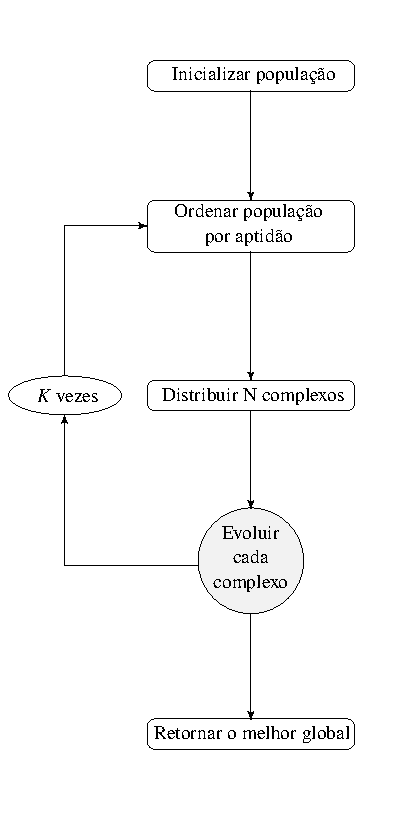
\includegraphics{imgs/flow1}
  \caption{The SCE algorithm.}
\end{figure}

\begin{figure}
  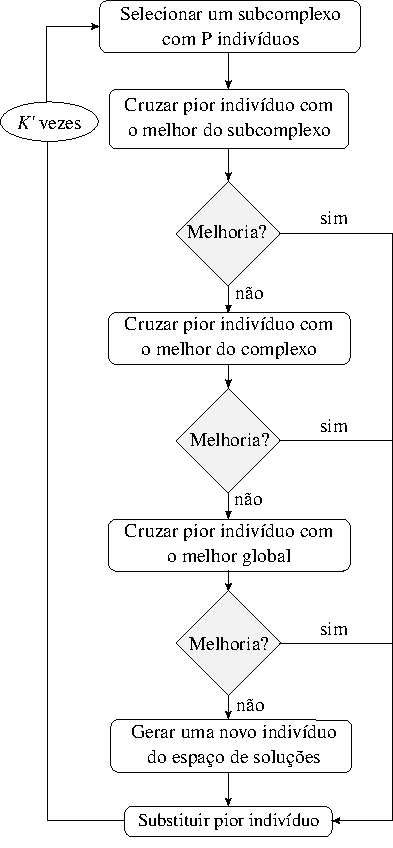
\includegraphics{imgs/flow2}
  \caption{The evolving procedure for a complex.}
\end{figure}


%\begin{algorithmic}
%  \Procedure{The SCE for the MKP}{$\vec{p}, W, \vec{b}$}
%    \State Inicialize population
%    \For{$ i \leftarrow 1:K$ }
%	  \State Sort population by fitness
%	  \State $s_{gb} \leftarrow$ Global best individual
%	  \State Shuffle complexes
%      \For{ each complex }
%	    \State $s_{cb} \leftarrow$ Complex best individual
%        \For{$ k \leftarrow 1:K'$ }
%		  \State Select a subcomplex of $P$ individuals
%          \State $s_w \leftarrow$ worst individual of subcomplex
%          \State $s_b \leftarrow$ best individual of subcomplex
%		  \State $s_{new} \leftarrow s_w \otimes s_b$
%		  \If{ $fitness(s_{new}) > s_w$}
%		    \State $s_w \leftarrow s_{new}$
%		  \Else
%		    \State $s_{new} \leftarrow s_w \otimes s_{cb}$
%		    \If{ $fitness(s_{new}) > s_w$}
%		      \State $s_w \leftarrow s_{new}$
%			\Else
%		      \State $s_{new} \leftarrow s_w \otimes s_{gb}$
%		      \If{ $fitness(s_{new}) > s_w$}
%		        \State $s_w \leftarrow s_{new}$
%		      \Else
%			    \State $s_w \leftarrow$ new random solution
%			  \EndIf
%		    \EndIf
%		  \EndIf
%        \EndFor
%      \EndFor
%    \EndFor
%	\State $s_gb \leftarrow$ Global best individual
%	\State Return $s_gb$
%  \EndProcedure
%\end{algorithmic}

%\begin{algorithmic}
%  \Procedure{New random MKP solution}{$\vec{p}, W, \vec{b}$}
%    \State $\vec{v} \leftarrow $ shuffle$(1, 2, \ldots, n)$
%	\State $s \leftarrow \emptyset $
%    \For{$ i \leftarrow 1:niter$ }
%	  \If{$ s \cup \{v[i]\} is feasible$}
%	    \State $s \leftarrow s \cup \{v[i]\}$
%	  \EndIf
%    \EndFor
%  \EndProcedure
%\end{algorithmic}

\section{Computational experiments}
\label{sec:exp}
% Instancias (tightness)
% parametros
% Gráficos:
%   - qualidade
%   - gráfico exemplificando o progresso durante as iterações.
% Futuro: testar cuzamentos de tipos diferentes e com mais individuos.

\section{Conclusions and future remarks}
\label{sec:conc}
% Conseguiu alcançar soluções "near optimal"

%\bibliographystyle{abbrv}
\bibliographystyle{IEEEtran}
\bibliography{../../refs}

%\printbibliography

\end{document}

